\section{Anwendungsschicht}

\paragraph{Historie}
\begin{itemize}
  \item \textbf{70er/80er}: Textbasierte Anwendungen (EMail, Remote Access)
  \item \textbf{90er}: World Wide Web, Instant Messaging, P2P-Filesharing
  \item \textbf{seit 2000}: steigende Vielfalt + Allgegenwärtigkeit: (\( \Rightarrow \) Kritische Infrastruktur) Voice over IP, Streaming, Gaming, Soziale Netzwerke, Smartphones
\end{itemize}

\paragraph{Schichtenmodell}
\begin{itemize}
  \item \textbf{Prozess}: Programm, das im Endsystem (Anwendungsschicht) abläuft
  \item \textbf{Nachricht}: Ausgetauscht zwischen Prozessen auf \emph{unterschiedlichen} Endsystemen
  \item Kommunikation in Schichten organisiert
  \item \textbf{Anwendungsschicht}: oberste Schicht
  \begin{itemize}
    \item enthält Anwendungsprotokolle
    \item Anwendung kümmert sich nicht um Datentransport
  \end{itemize}
  \item \textbf{Datentransport}: unter Anwendungsschicht liegende Schichten
  \begin{itemize}
    \item Interna für Anwendung transparent
    \item Aber: Anwendung merkt Verzögerungen (Latenzen)
  \end{itemize}
\end{itemize}

\paragraph{Verzögerung (Latenz)}
\begin{itemize}
  \item \textbf{Ausbreitungsverzögerung} \( t_a = \tfrac{d}{v} \)
  \begin{itemize}
    \item Zeitspanne zwischen Absenden eines Signals und dessen Eintreffen am anderen Ende des Mediums
    \item Abhängig von: Ausbreitungsgeschwindigkeit \( v \), Länge des Mediums \( d \)
  \end{itemize}
  \item \textbf{Sendezeit} \( t_s = \tfrac{X}{r} \)
  \begin{itemize}
    \item Zeit zwischen Beginn und Abschluss der Sendung
    \item Abhängig von: Datenmenge \( X \), Datenrate (Durchsatz) des Mediums \( r \)
    \item \textbf{Achtung}: Nach Sendungsabschluss sind die Daten noch nicht beim Empfänger! \( \leadsto \) Ausbreitungsverzögerung \( t_a \)
  \end{itemize}
  \item \textbf{Verzögerung im Router}:
  \begin{itemize}
    \item \emph{Pufferung} der Daten in Warteschlange
    \item \emph{Verarbeitung} (Fehlerüberprüfung usw.)
  \end{itemize}
\end{itemize}

\paragraph{Protokollstack}
\begin{itemize}
  \item \textbf{Application}: SMTP, HTTP, XMPP, \dots
  \item \textbf{Transport}: TCP, UDP
  \item \textbf{Network}: IP
  \item \textbf{Data Link}: Ethernet, 802.11 (WiFi)
  \item \textbf{Physical}: Bits auf Medium
\end{itemize}

\paragraph{Socket und Interface}
\begin{itemize}
  \item \emph{Programmierschnittstelle für verteilte Anwendungen}
  \item Von OS bereitgestellte API
  \item Anwendungsprozess sendet/empfängt Nachrichten zum/vom Socket
  \item \textbf{Portnummern}: (De-) Multiplexing auf Endsystemen, viele Prozesse auf einem Endsystem kommunizieren gleichzeitig über Netzwerk \\* \( \leadsto \) eindeutige Socket-Identifikation über Portnummer
\end{itemize}

\paragraph{Client-Server-Anwendungen}
\begin{itemize}
  \item \textbf{Server}: Ständig in Betrieb, permanente IP-Adresse, häufig in Datenzentren
  \item \textbf{Clients}: Kommunizieren mit Server, \emph{nicht} direkt miteinander, dyn. IP-Adresse
\end{itemize}

\paragraph{Peer-to-Peer-Anwendungen}
\begin{itemize}
  \item Endysteme kommunizieren direkt miteinander
  \begin{itemize}
    \item Fordern Dienste von anderen Peers an und stellen selbst Dienste bereit
    \item Nicht permanent verbunden, wechseln dynamisch IP-Adressen \\* \( \leadsto \) komplexes Management
  \end{itemize}
  \item \textbf{Selbstskalierend}: Neue Peers erhöhen Kapa, fordern aber auch Dienste an
\end{itemize}

\paragraph{Web und HTTP --- Web-Dokumente}
\begin{itemize}
  \item Webseiten bestehen aus HTML-Datei und anderen Objekten (.js, .png,\dots)
  \item Jedes Objekt über URL (\emph{uniform resource locator}) referenzierbar
\end{itemize}

\paragraph{HTTP (Hypertext Transfer Protocol)}
\begin{itemize}
  \item ASCII-basiertes Transferprotokoll der Anwendungsschicht im Web
  \item Basiert auf Client/Server-Modell
  \begin{itemize}
    \item \emph{Client (Request)}: Browser, der Web-Objekte anfordert
    \item \emph{Server (Response)}: Sendet über HTTP angeforderte Objekte
  \end{itemize}
  \item Zustandslos: Jeder Request individuell, keine Zustandsinformation auf Server
  \item Kommunikation per TCP:
  \begin{enumerate}
    \item Client initiiert Verbindungsaufbau (Standard-Port: 80)
    \item Server akzeptiert Verbindung
    \item Austausch von HTTP-Nachrichten
    \item Abbau der TCP-Verbindung
  \end{enumerate}
  \item HTTP-Anfragen können verschiedene \textbf{Methoden} nutzen:
  \begin{itemize}
    \item \textbf{GET}: Ressource von Server zu Client übertragen (z.B. normale Webseite)
    \item \textbf{POST}: Daten zu Ressource übertragen (z.B. Web-Formular)
    \item PUT: neue Ressource anlegen
    \item DELETE: Ressource löschen
    \item HEAD: wie GET, aber nur HTTP-Header übertragen
  \end{itemize}
  \item \textbf{Status-Codes:} Verarbeitungsindikator (Erfolg/Fehlschlag + Gründe)
  \begin{itemize}
    \item \textbf{200}: Erfolg; Antwort ist in dieser Nachricht
    \item \textbf{301}: Angefragtes Objekt verschoben (neue URL in Nachricht spezifiziert)
    \item \textbf{400}: Server hat Anfrage nicht verstanden
    \item \textbf{404}: Angefordertes Objekt existiert nicht
    \item \textbf{505}: HTTP-Version nicht unterstützt
  \end{itemize}
\end{itemize}
  \begin{figure}[H]\centering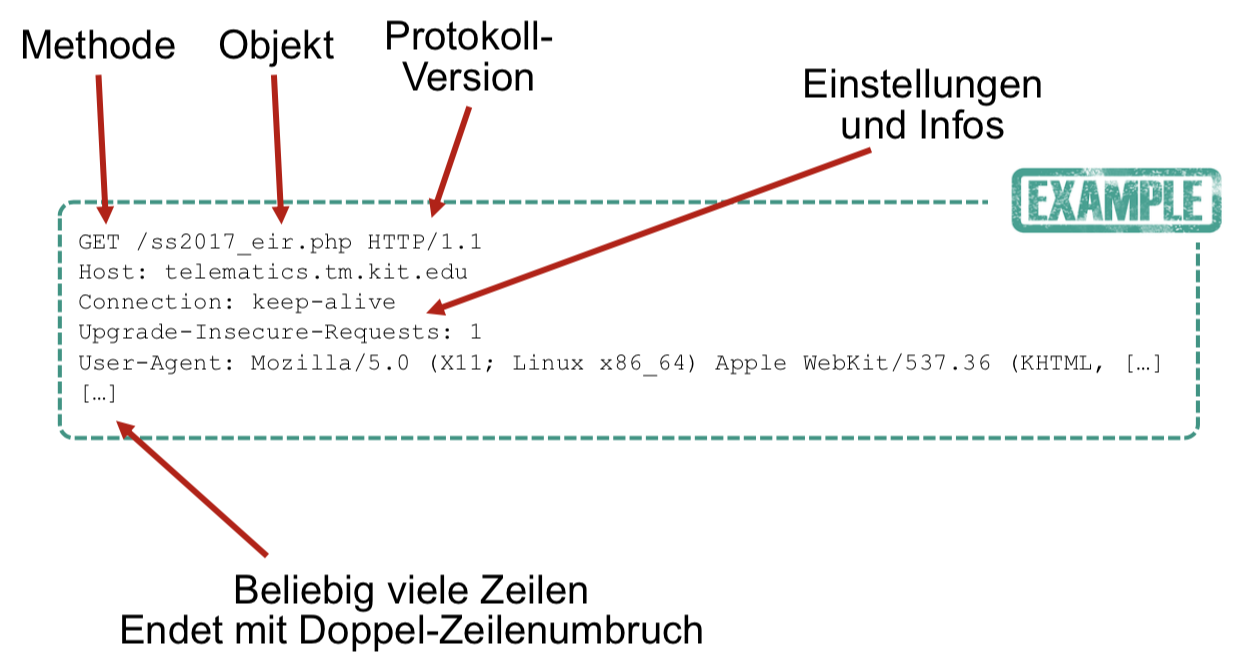
\includegraphics[width=0.33\textwidth]{HTTPRequest}\end{figure}
\begin{figure}[H]\centering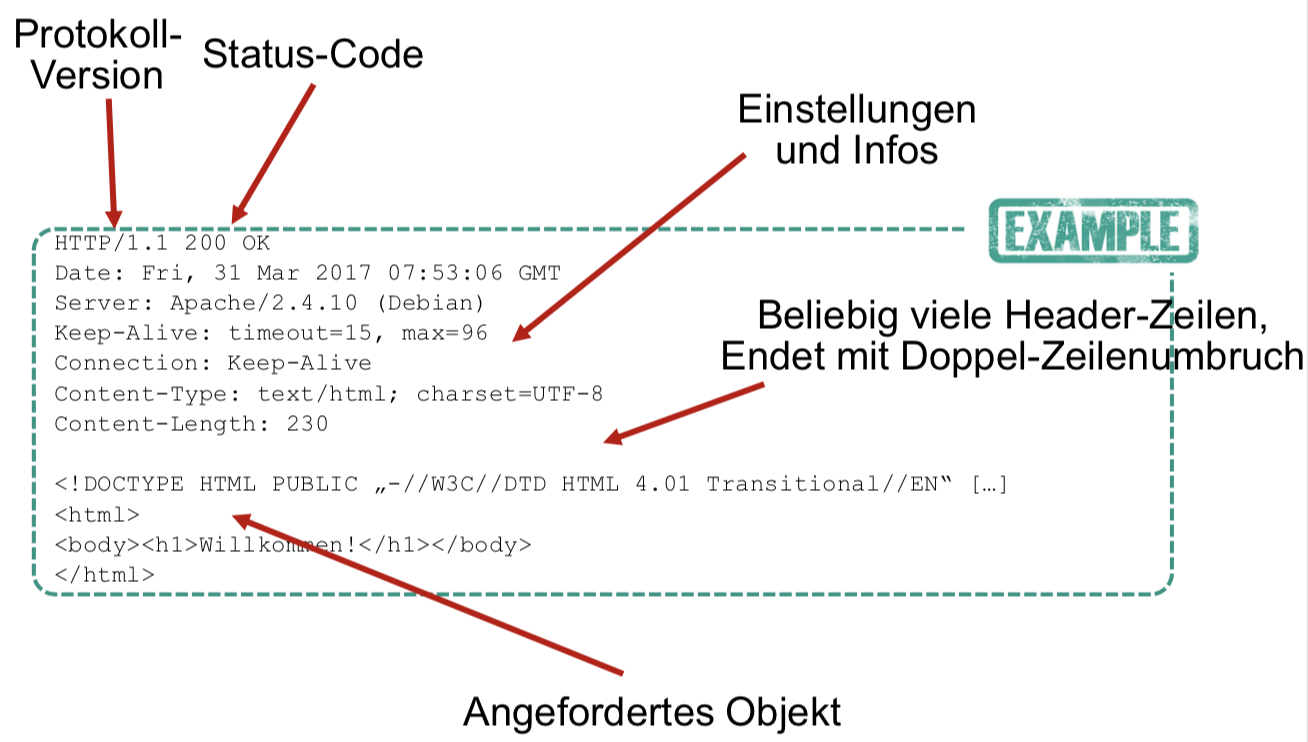
\includegraphics[width=0.33\textwidth]{HTTPResponse}\end{figure}

\paragraph{HTTP --- Verbindungen}
\begin{itemize}
  \item \textbf{Round Trip Time (RTT)}: Zeit, die Paket von Sender zu Empfänger und zurück benötigt
  \item \textbf{Non-persistent HTTP}: Höchstens ein Objekt über eine TCP-Verbindung, danach geschlossen \( \leadsto \) Mehrere Objekte erfordern mehrere TCP-Verbindungen (evtl. parallel)
  \begin{itemize}
    \item \emph{Antwortzeit}: \( 2*\text{RTT} + t_s \) pro Objekt (1 RTT Verbindungsaufbau, 1 RTT HTTP-Anfrage und erste Antwortbytes, \( t_s \) für Senden des Objekts)
  \end{itemize}
  \item \textbf{Persistent HTTP}: Mehrere Objekte über eine TCP-Verbindung
  \begin{itemize}
    \item \emph{Antwortzeit}: Nur eine RTT für nachfolgende Objekte
  \end{itemize}
\end{itemize}

\paragraph{HTTP --- Cookies}
\begin{itemize}
  \item \emph{Speichert Nutzer-Server-Zustand} \( \leadsto \) Server kann Inhalt pro Nutzer bereitstellen
  \item \textbf{Komponenten}:
  \begin{itemize}
    \item Cookie-Information in HTTP-Response-Nachricht (\textit{Set-Cookie})
    \item Cookie-Information wird in nachfolgenden HTTP-Requests genutzt
    \item Datei mit Cookies wird auf Nutzer-Endsystem vom Browser verwaltet
    \item Datenbank bei Webseite: Server muss Cookies richtig interpretieren können
  \end{itemize}
	\item \textbf{Privatsphäre: } Webseiten unterscheiden Nutzer durch Cookies \\*
    	\( \leadsto \) Werbeanbieter können Nutzer über viele Seiten tracken
\end{itemize}

\paragraph{Mail --- Komponenten}
\begin{itemize}
  \item \textbf{User Agent} (UA): Lesen, senden, weiterleiten
  \item \textbf{Mailserver}: User-Mailboxen, \emph{mail transfer/mail delivery agent} (MTA/MDA)
\end{itemize}

\paragraph{Mail --- SMTP (Simple Mail Transfer Protocol)}
\begin{itemize}
	\item Transfer von Mails zwischen Mailservern/von User Agent zu Mailserver
  \item \textbf{Phasen}: Handshake, Nachrichtenübermittlung (Header + Body), Abschluss
  \item Client/Server-Model, Command/Response-Interaktionen
  \begin{itemize}
    \item Ähnlich Request/Response bei HTTP, nutzt ebenfalls TCP (Port 25)
    \item Kommandos: ASCII-Text
    \item Antwort: Statuscode + Nachricht
  \end{itemize}
\end{itemize}

\paragraph{Mail --- MIME}
\begin{itemize}
  \item[=] \emph{Multipurpose Internet Mail Extensions}
  \item \textbf{Problem}: SMTP kann nur 7-Bit ASCII-Texte versenden, keine Dateien
  \item \textbf{MIME}: erweitert Kopfteil einer Nachricht um Formatinformation
  \item \textbf{Content-Type}: Definiert Typ des E-Mail-Inhalts; \emph{Content-Transfer-Encoding}
\end{itemize}

\paragraph{Mail --- Postfach-Abfrage}
\begin{itemize}
  \item \textbf{POP3} (\emph{post office protocol 3}): Verwaltung im UA, \emph{keine} Synchronisation
  \begin{itemize}
    \item Client holt am Mailserver gespeicherte Nachrichten ab
    \item nur einfache Funktionalität (\textit{list, retr, dele})
  \end{itemize}
  \item \textbf{IMAP} (\emph{interactive mail access protocol}): Zentrale Verwaltung auf Mailserver, erweiterte Kommandos (Ordner, Filter)
  \item \textbf{Web-Mail}
\end{itemize}

\paragraph{WhatsApp --- XMPP}
\begin{itemize}
  \item[=] \emph{eXtensible Messaging and Presence Protocol}, Echtzeit XML-Streaming
  \item Dezentral, ähnlich wie E-Mail
  \item Whatsapp nutzt Zentralen Server und proprietäre Variante des Protokolls
  \item \textbf{Clients}: zu ihrem jeweiligen Server verbunden
  \item \textbf{Server}: verbinden sich untereinander zur Nachrichtenübermittlung
  \item \textbf{Nachricht:} XML-Dokumente (erweiterbares Format)
  \item \textbf{Adressformat}: Server + Username, evtl. Client (z.B. alice@jabber.org/laptop)
\end{itemize}

\paragraph{DNS (Domain Name System)}
\begin{itemize}
  \item \textbf{Ziel}: Verwendung von Namen statt IP-Adressen
  \item \textbf{Aufgabe}: Zuordnung IP-Adresse \( \leftrightarrow \) Name (Subdomäne.Domäne.TLD)
  \item \textbf{Funktionalitäten}:
  \begin{itemize}
    \item \emph{Registrierung} von Namen + IP-Adressen
    \item \emph{Auflösung} von Namen in IP-Adressen
    \item \emph{Host Alias}: Löse einfachere Alias-Namen in kanonische Namen auf
    \item \emph{Mail Server Alias}: Liefere E-Mail-Server zu einer Domain
    \item \emph{Lastverteilung}: Mehrere IPs redundanter Server in zufälliger Reihenfolge
  \end{itemize}
  \item Protokoll der Anwendungsschicht, über UDP realisiert, Client-Server-Modell
  \item Basisdienst, keine eigentliche Anwendung: Komplexität am Rand des Netzes
\end{itemize}

\paragraph{DNS --- Aufbau}
\begin{itemize}
	\item Probleme mit zentralem Server: Singuläre Fehlerquelle, Verkehrsaufkommen, geografische Entfernung, Verwaltungsaufwand, Abhängigkeit
  \item Verteilte Datenbank in einer \textbf{Hierarchie} von Name-Servern (DNS-Servern)
  \begin{itemize}
    \item \emph{Lokaler NS}: Erste Anfrage immer zu lokalem Server, Antwort aus eigener Zuordnungsdatenbank, Cache oder nach Befragung anderer DNS-Server
    \item \emph{Autoritativer NS}: Enthält autoritative Abbildungen, jeder Host ist bei einem registriert (in seinem Netz)
    \item \emph{Top-Level Domain (TLD) Server}
    \item \emph{Root-Server}: Enthalten nur TLD-Einträge, fixe IPs, 13 Root-Server-Cluster
  \end{itemize}
\end{itemize}

\paragraph{DNS --- Anfragen}
\begin{itemize}
  \item \textbf{Rekursiv}: kennt angefragter Server Antwort nicht, fragt dieser weitere Server, bis er Antwort zurückliefern kann
  \item \textbf{Iterativ}: kennt Server die Antwort nicht, verweist er \emph{Client} an andere Server
  \item \textbf{Üblich}: Client fragt lokalen Name-Server rekursiv, dieser dann iterativ
\end{itemize}

\paragraph{DNS --- Resource Records (RR)}
\begin{itemize}
  \item DNS ordnet Domänen zu Einträgen zu
  \item \textbf{A / AAAA} (Address): Abbildung Name auf IPv4/IPv6-Adresse
  \item \textbf{MX} (Mail Exchange): Mailserver einer Domäne (IP-Adresse)
  \item \textbf{NS} (Name Server): Nameserver einer Domäne (Hostname)
  \item \textbf{CNAME} (Canonical Name): Alias-Namen für Rechner/Domänen (Domain)
  \item \textbf{PTR} (Pointer): Abbildung IP-Adresse auf Name (Domain)
\end{itemize}

\paragraph{Content Delivery Networks (CDN)}
\begin{itemize}
	\item \textbf{Beispiel: Videostreaming} (hohe Datenrate, Datenqualität)
	\item \textbf{DASH (Dynamic, Adaptive Streaming over HTTP)}: Video aufgeteilt in Chunks, jeweils in mehreren Qualitäten (Bitraten) verfügbar, URLs und Infos in Manifest-Datei\\*
	Client wählt adaptiv bestmögliche Bitrate für jeden Chunk
	\item \textbf{Content Distribution}: Content zu hunderttausend Nutzern bringen
	\item Mega-Server: Skaliert nicht (Single Point of Failure, Netzwerküberlastung, Entfernung)
	\item \textbf{CDN:} Content auf geographisch verteilte Server kopieren\\*
		Third-Party CDNs (z.B. Akamei, Limelight), Private CDNs (z.B. Google für YouTube)
	\item \textbf{Strategien}:
	\begin{itemize}
    \item \emph{enter deep}: Viele kleine Cluster in Zugangsnetzen nahe beim Nutzer
    \item \emph{bring home}: Wenige große Cluster in wichtigen IXPs für geringeren Verteilungs- und Wartungsaufwand
  \end{itemize}
	\item DNS-Manipulation: Autoritativer DNS-Server des CDN passt Antwort an IP-Adresse des anfragenden lokalen DNS-Server an, wählt einen nahe gelegenen CDN-Server aus
\end{itemize}